%% REPLACE sXXXXXXX with your student number
\def\studentNumber{s1803764}


%% START of YOUR ANSWERS
%% Add answers to the questions below, by replacing the text inside the brackets {} for \youranswer{ "Text to be replaced with your answer." }. 
%
% Do not delete the commands for adding figures and tables. Instead fill in the missing values with your experiment results, and replace the images with your own respective figures.
%
% You can generally delete the placeholder text, such as for example the text "Question Figure 2 - Replace the images ..." 
%
% There are 19 TEXT QUESTIONS (a few of the short first ones have their answers added to both the Introduction and the Abstract). Replace the text inside the brackets of the command \youranswer with your answer to the question.
%
% There are also 3 "questions" to replace some placeholder FIGURES with your own, and 3 "questions" asking you to fill in the missing entries in the TABLES provided. 
%
% NOTE! that questions are ordered by the order of appearance of their answers in the text, and not by the order you should tackle them. Specifically, you cannot answer Questions 2, 3, and 4 before concluding all of the relevant experiments and analysis. Similarly, you should fill in the TABLES and FIGURES before discussing the results presented there. 
%
% NOTE! If for some reason you do not manage to produce results for some FIGURES and TABLES, then you can get partial marks by discussing your expectations of the results in the relevant TEXT QUESTIONS (for example Question 8 makes use of Table 1 and Figure 2).
%
% Please refer to the coursework specification for more details.


%% - - - - - - - - - - - - TEXT QUESTIONS - - - - - - - - - - - - 

%% Question 1: define overfitting
\newcommand{\questionOne} {
\youranswer{when a model learns the ”noise” in the training data and becomes too specific so that it does not do well when generalizing to new unseen data}
}

%% Question 2: Summarise the effect increasing width and depth of the architecture had on overfitting
\newcommand{\questionTwo} {
\youranswer{improves the validation accuracy but worsens the validation error, this indicates that our model is overfitting to "noise" in the training set and thus implies that we should stop training earlier (when the validation accuracy is at it's maximum), and apply regularisation techniques to penalise large weights and ultimately reduce the complexity of the model}
}
%helps until the number of parameters becomes too high so that each layer just memorizes the training data, and you can end up with a neural network that fails to generalize well to new unseen data

%% Question 3: Summarise what your results show you about the effect of the tested approaches on overfitting and the performance of the trained model
\newcommand{\questionThree} {
\youranswer{%dropout was the best technique as it produced the best performing model with 84.45\% validation accuracy at a probability of 0.9. Out of the weight penalty techniques L1 regularisation produced the best model with 84.22\% validation accuracy using a coefficient of 1e-4.
dropout is the most effective regularisation technique for mitigating overfitting as it does a bit more than just regularisation and actually adds robustness to the network. This is due to the usage of deactivated neurons (which are ignored in the forward and backward propagations) which effectively compares our network with various different ones (given that deactivating neurons acts as a way to randomly change the dimensions of each layer) and chooses the best one. Although, the L1 and L2 regularisation techniques did not produce a validation accuracy as good as that of dropout, they did produce the best generalisation gaps and came very close to the performance produced by dropout
%as it forces nodes within a layer to probabilistically take on more or less responsibility for the inputs.s, for all combinations of hidden units and layers dropout always improved performance.
} 
}

%% Question 4: Give your overall conclusions
\newcommand{\questionFour} {
\youranswer{Q4}
}

%% Question 5: Explain what overfitting is in detail and in your own words
\newcommand{\questionFive} {
\youranswer{it is trained for too long resulting in an increasingly large generalization gap (the difference between the training error and validation error) and a decreasing validation accuracy. These trends indicate that the model is starting to learn "noise" in the training data and thus hinders the model's ability to generalize well to new unseen data such as the validation set}
}

%% Question 6: Discuss ``why'' and ``how'' overfitting occurs, and ``how'' one can identify it is happening
\newcommand{\questionSix} {
\youranswer{Overfitting occurs due to the mathematical techniques we use to train and optimise our ML models. In order to optimise our model we define an error function that represents how far our model's predictions are away from the real labels, thus to create a model with perfect accuracy we want a model that produces 0 error. So in order to minimize the error of our model we can try adjust the weights of our model that moves our error function towards a local/global minimum (by finding where the derivative of this error function is equal to 0). However, the problem here is that this error function is defined by the training data which inevitably stores some "noise" due to various reasons (data collection errors; due to inaccurate/miscalibrated sensors, or varying conditions; or noise added by computer processing such as floating point round-off errors etc.), and so as we begin to become close to 0 error we start to fit this "noise" into our model. Thus we must be wary as to when we should stop training our model to prevent fitting this "noise". We can identify when our model starts to overfit when the generalisation gap starts to increase and the validation accuracy starts to decrease, as this indicates that this further training is actually worsening the performance of this model
}
}

%% Question 7: Explain what these figures contain and how the curves evolve, and spot where overfitting occurs. Reason based on the min/max points and velocities (direction and magnitude of change) of the accuracy and error curves
\newcommand{\questionSeven} {
\youranswer{
the training and validation accuracies both improve logarithmically with the number of epochs, however, after epoch 17 we can see that the validation accuracy begins to decrease linearly with the number of epochs. This indicates that this model is starting to overfit to the "noise" in the training set after epoch 17 as the validation accuracy starts to decrease and generalisation gap starts to increase with the number of epochs.
This is further supported by figure~\ref{fig:example_errorcurves} which shows the validation and training errors as we increase the number of epochs. We can see that after epoch 17 the validation error starts to slowly increase in a linear fashion and the generalisation gap ($E_{train} - E_{valid}$) starts to increase exponentially (due to the fact that the training error continues to decrease linearly and the validation error continues to increase linearly).
%, thus if we were given this figure when choosing the optimal model we would choose the model at epoch 17 as this gives the best validation set performance. We see that figure 1b appears like figure 1a flipped upside down, this is to be expected given these graphs are reporting the opposite metrics.
}
}

%% Question 8: Explain your network width experiment results by using the relevant figure and table
\newcommand{\questionEight} {
\youranswer{as given by table~\ref{tab:width_exp} the widest model (128 units) performed the best given it produced the best validation accuracy, however, it was also the most overfitted given it produced the largest generalization gap.
This seems to be the general trend for these width experiments, that as we increase the width of our model, our validation accuracy and generalization gap both increase. 
This is evident from both figure~\ref{fig:width_acccurves} and figure~\ref{fig:width_errorcurves}. In figure~\ref{fig:width_acccurves} we can see that the validation accuracy of the model with 128 units peaks at epoch 20 and after this it decreases slowly in a linear fashion with the number of epochs and converges with the validation accuracies of the thinner models. In figure~\ref{fig:width_errorcurves} we can see that the classification error of the model with 128 units reaches its minimum at epoch 9 and after this it increases slowly as the training error continues to decrease with the number of epochs, indicating a widening of the generalization gap.
From these figures we can also see that these thinner models do not overfit as quickly as the wider ones due to their lower complexity. This lower complexity implies that these thinner networks are not able to store as much information as the wider networks making it harder for them to fit to the training data and thereby store the insignificant features/"noise" from the training data. This is evident in figure~\ref{fig:width_acccurves} as the model with 32 units continues to slowly increase in validation accuracy all the way up to epoch 94 (where it reaches it's maximum validation accuracy) in contrast to the 128 unit model which achieved maximum validation accuracy at epoch 20, and the 64 unit model which achieved maximum validation accuracy at epoch 29. These exponential differences between the optimal epoch numbers for each model are to be expected given the exponential differences in the widths of all these models ($32 = 2^5$, $64 = 2^6$, and $128 = 2^7$)
%The large differences in validation accuracies seen in figure \ref{fig:depth_acccurves} at around epoch 20 are a direct indication of how increasing the width of a model can increase it's performance.
%Given the results from table~\ref{tab:width_exp} alone, if I had to choose one of these models (that was trained for 100 epochs) for implementation I would choose the model with 64 units width. Although it has a slightly worse validation accuracy than that of the 128 unit model it has a far better generalization gap implying it will be a better model for generalizing to new unseen data
%the width of our model is directly proportional to validation accuracy until a certain epoch at which the model begins to become overfitted (given the validation accuracy starts to decrease and the generalization gap starts to increase). This is evident from figure 2a in which you can see that the validation accuracy of the model with 128 units peaks at epoch 20 and after this it decreases slowly and converges with the validation accuracies of the thinner models. We can see that these thinner models do not overfit as quickly as this one due to their lower complexity, this is evident in the graph as the model with 32 units continues to slowly increase in validation accuracy all the way up to epoch 94 (where it reaches it's maximum validation accuracy). From table 1 we can see that the model with 128 units is overfitted due it's near identical validation accuracy with the 64 unit model yet far larger generalization gap
}
}

%% Question 9: Discuss whether varying width affects the results in a consistent way, and whether the results are expected and match well with the prior knowledge (by which we mean your expectations as are formed from the relevant Theory and literature)
\newcommand{\questionNine} {
\youranswer{
%From these results it is evident that varying widths in this neural network architecture affected the results in a consistent way. We know that the larger the width of a model implies a larger complexity and thereby a higher susceptibility to overfitting. Thus as we increased the width of the models they became more susceptible to overfitting and so achieved their peak validation accuracies at much lower epochs. Thus table 1 is rather misleading in the quality of varying widths, as all these metrics were scored after training each model for 100 epochs rather than training each model for their optimal number of epochs.
From these results it is evident that as we increase the width of our model the validation accuracy increases, the classification error decreases, and the number of epochs needed to train our model decreases. However, we must note that this observation only holds up when we stop training our model before it becomes overfitted. We can define this point of overfitting to be the epoch when the given model reaches their optimum validation accuracy as this indicates this model is best at generalising to new unseen data. This overfitting is due to the fact that as we increase the number of training epochs our error function comes closer and closer to reaching a local minimum, but this local minimum is defined by the training samples in our dataset and thus as we get closer to this minimum our network starts to fit noise from our training data preventing it from being able to generalise well. This overfitting is evident across all our models here as they all reach their maximum validation accuracy scores before epoch 100, and after the epoch where this maximum validation accuracy is achieved we can see that for each model the validation accuracy starts to slowly decrease and the classification error starts to slowly increase.
These results were to be expected as the wider the model implies more information can be stored in the network allowing it to make more informed predictions. Furthermore, being able to store more information can also make the model more susceptible to overfitting as if it is trained for too long it can result in the network storing the "noise" from the training data and thus not allowing it to generalize well to new unseen data, which explains why the wider models overfit more quickly than shallower ones
}
}

%% Question 10: Explain your network depth experiment results by using the relevant figure and table
\newcommand{\questionTen} {
\youranswer{
as given by table~\ref{tab:depth_exps} the deepest model (3 layers) performed the best given it produced the best validation accuracy, however, it was also the most overfitted given it produced the largest generalization gap.
This seems to be the general trend for these depth experiments, that as we increase the depth of our model, our validation accuracy and generalization gap both increase. 
This is evident from both figure~\ref{fig:depth_acccurves} and figure~\ref{fig:depth_errorcurves}. In figure~\ref{fig:depth_acccurves} we can see that the validation accuracy of the model with 3 layers peaks at epoch 11 and after this it decreases slowly in a linear fashion with the number of epochs and converges with the validation accuracies of the shallower models. In figure~\ref{fig:depth_errorcurves} we can see that the classification error of the model with 3 layers units reaches its minimum at epoch 7 and after this it increases slowly as the training error continues to decrease with the number of epochs, indicating a widening of the generalization gap.
From these figures we can also see that these shallower models do not overfit as quickly as the deeper ones due to their lower complexity. This lower complexity implies that these shallower networks are not able to store as much information as the deeper networks making it harder for them to fit to the training data and thereby store the insignificant features/"noise" from the training data. This is evident in figure~\ref{fig:depth_acccurves} as the model with 1 layer continues to slowly increase in validation accuracy all the way up to epoch 20 (where it reaches it's maximum validation accuracy) in contrast to the 3 layer model which achieved maximum validation accuracy at epoch 11, and the 2 layer model which achieved maximum validation accuracy at epoch 17. These linear differences between the optimal epoch numbers for each model are to be expected given the linear differences in the depths of all these models
%as given by table~\ref{tab:depth_exps} the deepest model (3 layers) performed the best given it produced the best validation accuracy, however, it was also the most overfitted given it produced the largest generalization gap.
%This seems to be the general trend from these depth experiments, that as we increase the depth of our model, our validation accuracy and generalization gap both increase. 
%This is evident from figure~\ref{fig:depth_acccurves} in which you can see that the validation accuracy of the model with 3 layers peaks at epoch 11 and after this it decreases slowly and converges with the validation accuracies of the thinner models. We can see that these shallower models do not overfit as quickly as this one due to their lower complexity, this is evident in the graph as the model with 1 layer continues to slowly increase in validation accuracy all the way up to epoch 20 (where it reaches it's maximum validation accuracy).
%Given the results from table~\ref{tab:depth_exps} alone, if I had to choose one of these models (that was trained for 100 epochs) for implementation I would choose the model with 3 layers. Although it has the worst generalization gap this model achieved the best validation accuracy performing almost 1\% better than the model with 2 layers
}
}

%% Question 11: Discuss whether varying depth affects the results in a consistent way, and whether the results are expected and match well with the prior knowledge (by which we mean your expectations as are formed from the relevant Theory and literature)
\newcommand{\questionEleven} {
\youranswer{From these results it is evident that as we increase the depth of our model the validation accuracy increases, the classification error decreases, and the number of epochs needed to train our model decreases. However, we must note that this observation only holds up when we stop training our model before it becomes overfitted. We can define this point of overfitting to be the epoch when the given model reaches their optimum validation accuracy as this indicates this model is best at generalising to new unseen data. This overfitting is due to the fact that as we increase the number of training epochs our error function comes closer and closer to reaching a local minimum, but this local minimum is defined by the training samples in our dataset and thus as we get closer to this minimum our network starts to fit noise from our training data preventing it from being able to generalise well. This overfitting is evident across all our models here as they all reach their maximum validation accuracy scores long before epoch 100, and after the epoch where this maximum validation accuracy is achieved we can see that for each model the validation accuracy starts to slowly decrease and the classification error starts to slowly increase.
These results were to be expected as the deeper the model implies more information can be stored in the network allowing it to make more informed predictions. Furthermore, being able to store more information can also make the model more susceptible to overfitting as if it is trained for too long it can result in the network storing the "noise" from the training data and thus not allowing it to generalize well, which explains why the deeper models overfit more quickly than shallower ones
}
}

%% Question 12: Compare and discuss how varying width and height changes the performance and overfitting in your experiments
\newcommand{\questionTwelve} {
\youranswer{
From table~\ref{tab:width_exp} and table~\ref{tab:depth_exps} we can see that increasing depth is a more effective means to increase performance as it achieves better validation accuracy across all models (when looking at the optimal validation accuracy across 100 epochs). We can also see from these tables that increasing width makes the model less susceptible to overfitting than increasing the depth given the far smaller generalization gaps achieved across all the width experiment models. When looking at figure \ref{fig:width_acccurves} and figure \ref{fig:depth_acccurves} we can see that there is a far larger gap in accuracies between the models of varying width which indicates the rapid improvement increasing width can have on a model's performance. 
Finally, when analysing these two methods for developing neural networks we must also keep in mind the computational costs of each of these, as different applications may demand different amounts of computational efficiency. In a time-critical application (where computation speed needs to be minimised as much as possible) it is more computationally effective to widen the network than increase the depth of the network as wider networks allow many multiplications to be completed in parallel, unlike deeper networks which require more sequential operations (since the computations depend on the outputs of the previous layers) \cite{DBLP:journals/corr/ZagoruykoK16}
}
}

%% Question 13: Explain L1/L2 weight penalties first in words and then with formulas. Explain how they are incorporated to training and what hyperparameter(s) they require
\newcommand{\questionThirteen} {
\youranswer{
These techniques work by adding a regularization term to the error function which acts as a penalty for complex models with large weights. This is so that when we train our model using gradient descent, our error function will gravitate towards a local minimum that does not take "noisy"/insignificant features into account. The mathematical formula for the error function without regularization is as follows:
$$ E^n = E^{n}_{train}$$
\\
\\
We incorporate L1 regularisation into training our model  by adding a regularisation term to this error function that penalizes large weights: 
%L1 regularisation is the preferred choice when having a high number of features as it provides sparse solutions. In L1 the weights shrink to 0 at a constant rate ($\beta \text{sgn}(w_i)$), thus the new mathematical formula for the loss function with L1 regularization is as follows:
$$ E^n = E^{n}_{train} + \beta \sum_{i=1}^{n}|w_i|$$
$$ \text{where } \beta \text{ is the regularization parameter}$$

And now we can try to reach the \emph{new} local/global minimum of our L1 error function by using the following equation:

$$ \frac{\partial E^n}{\partial w_i} = \frac{\partial E_{train}^{n}}{\partial w_i} + \beta \text{sgn}(w_i)$$
$$\text{where } \text{sgn}(w_i) \text{ is the sign of }w_i$$ 
\\
\\
%This added regularisation term evidently indicates that L1 regularisation penalizes the weights of a model by calculating the sum of the absolute value of the weights 
%L2 regularisation can deal with multicollinearity (independent variables that are highly correlated) problems through constricting the coefficient and by keeping all the variables. L2 regression can be used to estimate the significance of predictors and based on that it can penalize the insignificant predictors. In L2 weights shrink to 0 at a rate proportional to the size of the weight ($ \beta w_i$), 
We incorporate L2 regularisation into training our model  by adding a regularisation term to this error function that penalizes large weights: 
$$ E^n = E^{n}_{train} + \beta \sum_{i=1}^{n}w_i^2 $$
$$ \text{where } \beta \text{ is the regularization parameter} $$

And now we can try to reach the \emph{new} local/global minimum of our L2 error function by using the following equation:
$$ \frac{\partial E^n}{\partial w_i} = \frac{\partial E_{train}^{n}}{\partial w_i} + \beta w_i$$
\\

This regularization parameter $\beta$ is evidently extremely important to both these regularization techniques as it directly affects the complexity and training-data fit of the model. Given this parameter is handpicked it is extremely important that it is set optimally. The choice of this parameter is entirely dependent on how far we want to simplify our model (as increasing it's magnitude strengthens this regularization effect) so we must keep the initial performance and fitting of our model in mind when choosing this. As shown in table~\ref{tab:hp_search} a good method to choose this parameter would be to test varying size $ \beta$ values on the validation set and choose the one that produces the best validation accuracy
}
}

%% Question 14: Discuss how/why the weight penalties may address overfitting, discuss how L1 and L2 regularization differ and support your claims with references where possible
\newcommand{\questionFourteen} {
\youranswer{
These regularisation techniques address overfitting by penalising large weights in models. Penalising these large weights helps to reduce the complexity of the model and ultimately retain less noise from the training set. The main difference between L1 and L2 regularisation is the regularisation terms they add to the error function. In L1 regression weights shrink to 0 at a constant rate ($\beta \text{sgn}(w_i)$) in contrast to L2 regression where weights shrink to 0 at a rate proportional to the magnitude of the weight ($\beta w_i$). This difference is due to the fact that L1 regularization penalizes the sum of the absolute value of weights whereas L2 regularization penalizes the sum of square weights. Such differences in these regularization terms give each of these methods different strengths for different types of data. L1 regularisation is particularly useful for feature selection as it produces a sparse solution and allows us to drop features based on the weights that go to 0 \cite{neelam_tyagi_2021}. L2 regularisation on the other hand produces non-sparse solutions and is useful when you have collinear/codependent features in your dataset. This is due to the fact that codependence tends to increase weight variance, which makes the weights unreliable/unstable and can end up hurting the model's generality. L2 fixes this by reducing the variance of these estimates which counteracts the effect of codependencies \cite{explained_regularization_2021}
}
}

%% Question 15: Explain the experimental details (e.g. hyperparameters), discuss the results in terms of their generalization performance and overfitting
\newcommand{\questionFifteen} {
\youranswer{
From our Dropout experiments it is evident to see that validation accuracy and generalisation gap are both directly proportional to the Dropout probability when $0.7 <= p <= 0.95$ (where $p$ is the Dropout probability). This was achieved by applying a Dropout layer before each Affine layer in our network, using the same Dropout probability for each Dropout layer. 

However, these results do not cover any cases where the dropout probability is less than 0.5, this is problematic as we cannot extrapolate these results from our 3 experiments, rather we need to test them.

For my combined regularisation method experiments I carefully chose what hyperparameters to use. From the Dropout experiments it was evident that setting the Dropout probability to 0.95 was the optimal choice since it gave the highest validation accuracy of 86.15\%. Thus for all my combination experiments I decided to keep the Dropout probability fixed at 0.95 to maximise validation accuracy. Now the only hyperparameter left to choose were the weight penalty techniques and their coefficients.

For my combined I varied the dropout probabilities across the different layers to maximise validation accuracy
}
}

%% Question 16: Explain the motivation behind Maxout Networks as presented in \cite{goodfellow2013maxout}
\newcommand{\questionSixteen} {
\youranswer{
it has not previously been demonstrated to actually perform model averaging for deep architectures. Dropout is generally seen as an indiscriminately applicable tool that
maxout networks are designed to both facilitate optimisation by dropout and improve the accuracy of dropout's fast approximate model averaging technique.
The maxout network is a feed-forward architecture that uses a new type of activation function called the maxout unit. Given an input a maxout hidden layer implements the following function:
$$ h_i(x) = \max_{j \in [1,k]} z_{ij} $$
$$\text{where } z_{ij}=x^T W_{...ij} + b_{ij} \text{ , and } W \in \mathbb{R}^{d \times m \times k} \text{ and } b \in \mathbb{R}^{m \times k}$$
$$\text{ are learned parameters}$$

A single maxout unit can be interpreted as making a piecewise linear approximation to an arbitrary convex function. Maxout networks learn not just the relationship between hidden units, but also the activation function of each hidden unit. A multilayer perceptron containing 2 maxout units can be used to arbitrarily approximate any function
}
}

%% Question 17: State whether Dropout is compatible (can be used together) with Maxout and explain why
\newcommand{\questionSeventeen} {
\youranswer{
We know that Dropout is compatible with Maxout given Maxout was developed as a method to enhance Dropout's abilities as a model averaging technique. This is further supported by the founding paper on Maxout networks \cite{goodfellow2013maxout} which actually used Maxout in conjunction with Dropout to test Maxout's performance on benchmark datasets
}
}

%% Question 18: Give an overview of the experiment setup in \cite{goodfellow2013maxout} and analyse it from the point of view of how convincing their conclusions are 
\newcommand{\questionEighteen} {
\youranswer{
The setup was good as they decided to test their novel method on benchmark datasets.

However, I believe they should have provided error scores for models fitted with Dropout alone, and with Maxout alone. As althought they said it was "particularly well suited for training with dropout" it is still useful to be able to compare these metrics.

In the conclusion it was stated that Maxout exploits model averaging behaviour because the approximation is more accurate for Maxout units than for tanh units. However, there are many other units than tanh units that this method could have been compared against.

They decided to make a proof that proves Maxout is a universal approximator, this is a good method as it ensures conservation of logic.
}
}

%% Question 19: Briefly draw your conclusions based on the results from the previous sections (what are the take-away messages?) and conclude your report with a recommendation for future directions
\newcommand{\questionNineteen} {
\youranswer{Q19

In the future, to optimise these models even further there are a number of things we could do. Such as optimise the depth and width of our model even further, choose the optimal activation function, optimise the structure of the Dropout layers in our architecture, optimise the L1/L2 regularization parameters even further, and optimise the random seed used to initialize our weights, and Dropout layers. 


Firstly, to optimise this Dropout model even further we could optimise the number of Dropout layers used, their placement within the network (before which Affine layers), and the Dropout probabilities used for each of these layers.

Secondly, to optimise the L1 and L2 regularization models even further we could optimise the regularisation parameter for the weights and bias separately.

Thus to optimise our combination experiments in the future we could use the new results from our experiments described above as a way to structure our neural network architecture optimally. I would also like to test 
}
}


%% - - - - - - - - - - - - FIGURES - - - - - - - - - - - - 

%% Question Figure 2:
\newcommand{\questionFigureTwo} {
\youranswer{%Question Figure 2 - Replace the images in Figure 2 with figures depicting the accuracy and error, training and validation curves for your experiments varying the number of hidden units.
%
\begin{figure}[t]
    \centering
    \begin{subfigure}{\linewidth}
        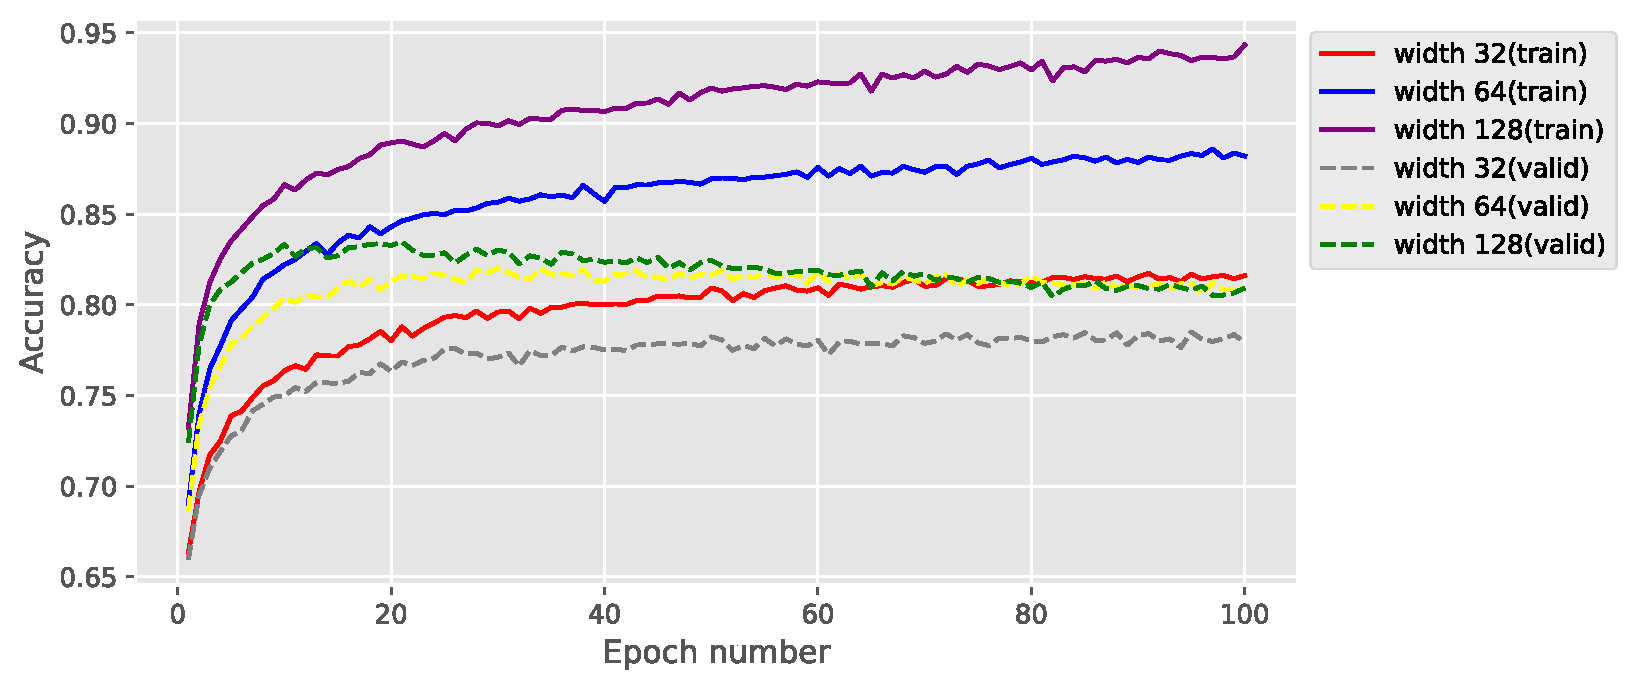
\includegraphics[width=\linewidth]{figures/width-fig1.pdf}
        \caption{accuracy by epoch}
        \label{fig:width_acccurves}
    \end{subfigure} 
    \begin{subfigure}{\linewidth}
        \centering
        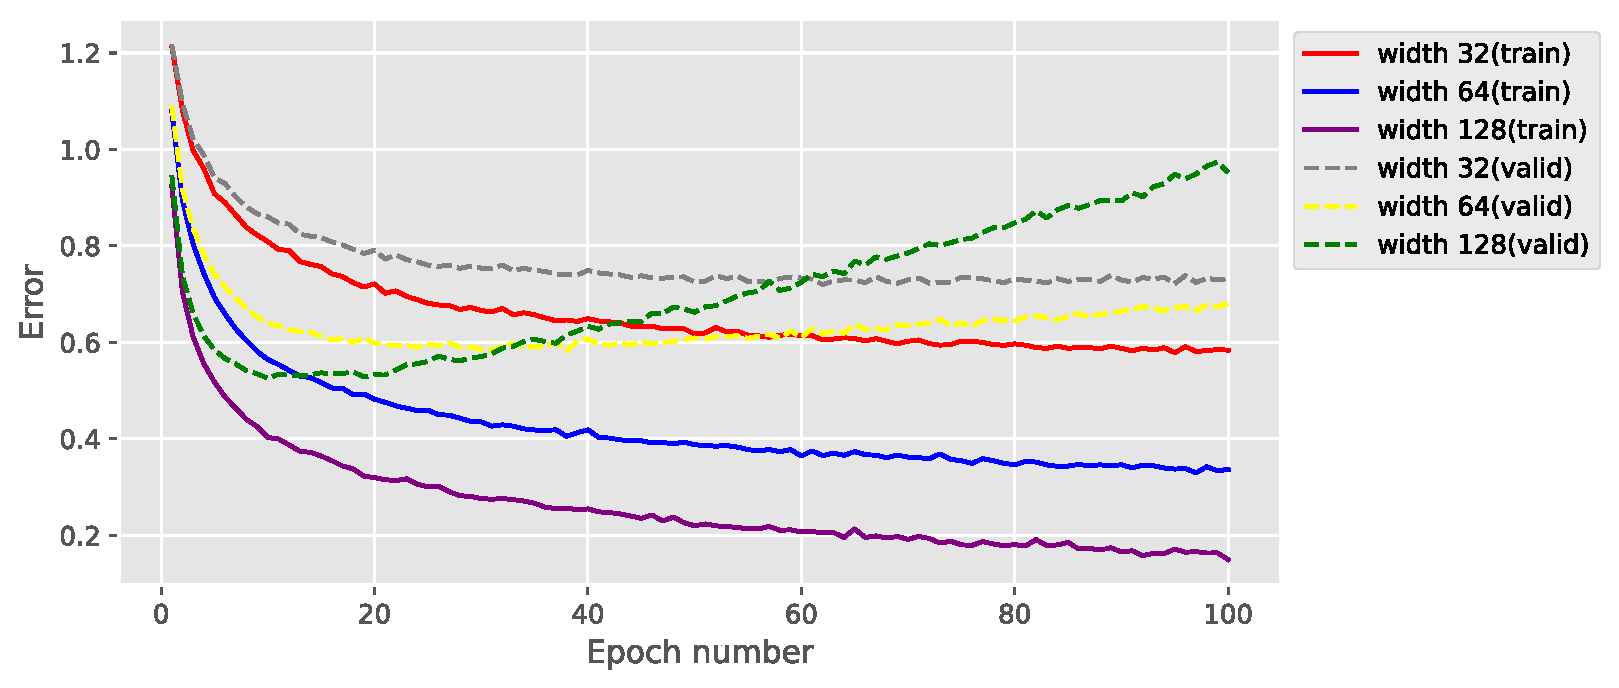
\includegraphics[width=\linewidth]{figures/width-fig2.pdf}
        \caption{error by epoch}
        \label{fig:width_errorcurves}
    \end{subfigure} 
    \caption{Training and validation curves in terms of classification accuracy (a) and cross-entropy error (b) on the EMNIST dataset for different network widths.}
    \label{fig:width}
\end{figure} 
}
}

%% Question Figure 3:
\newcommand{\questionFigureThree} {
\youranswer{%Question Figure 3 - Replace these images with figures depicting the accuracy and error, training and validation curves for your experiments varying the number of hidden layers.
%
\begin{figure}[t]
    \centering
    \begin{subfigure}{\linewidth}
        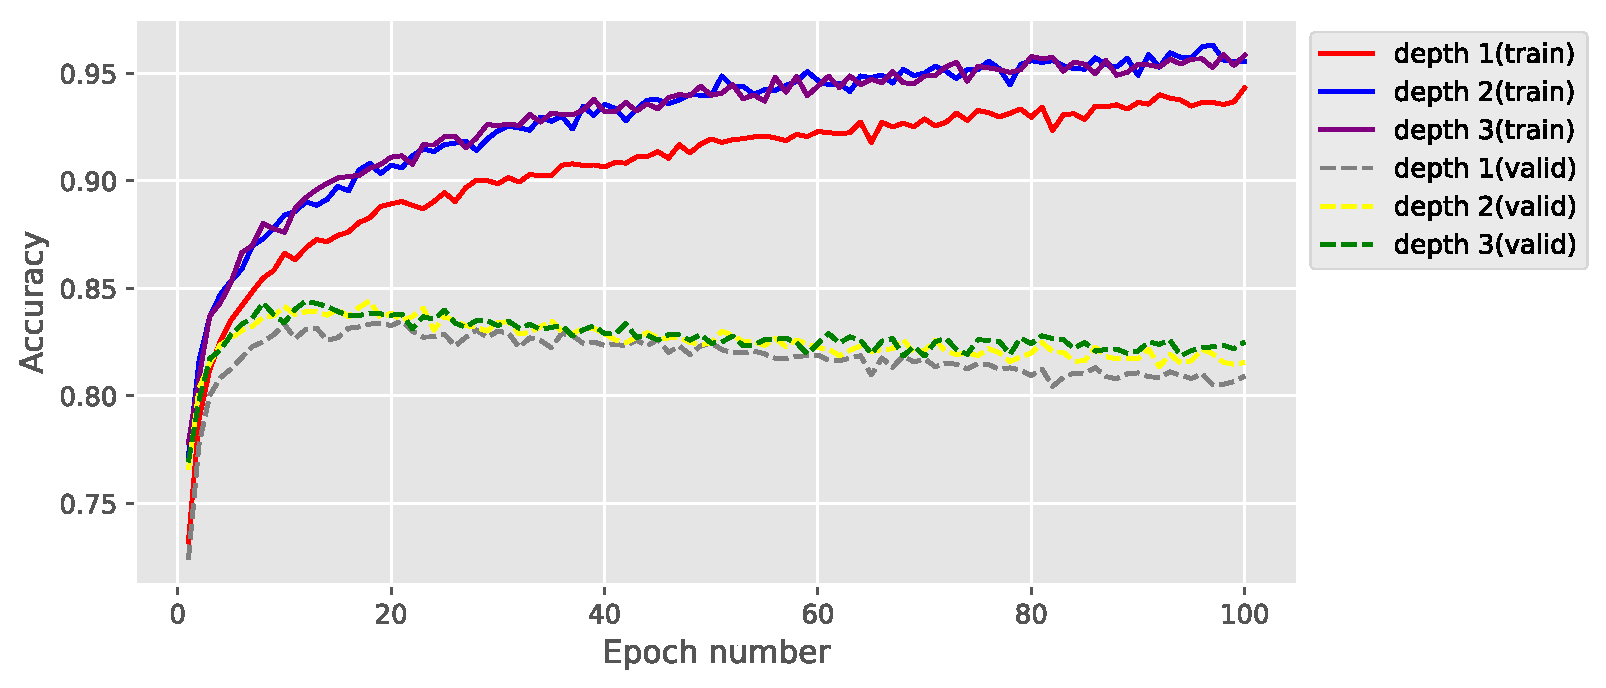
\includegraphics[width=\linewidth]{figures/depth-fig1.pdf}
        \caption{accuracy by epoch}
        \label{fig:depth_acccurves}
    \end{subfigure} 
    \begin{subfigure}{\linewidth}
        \centering
        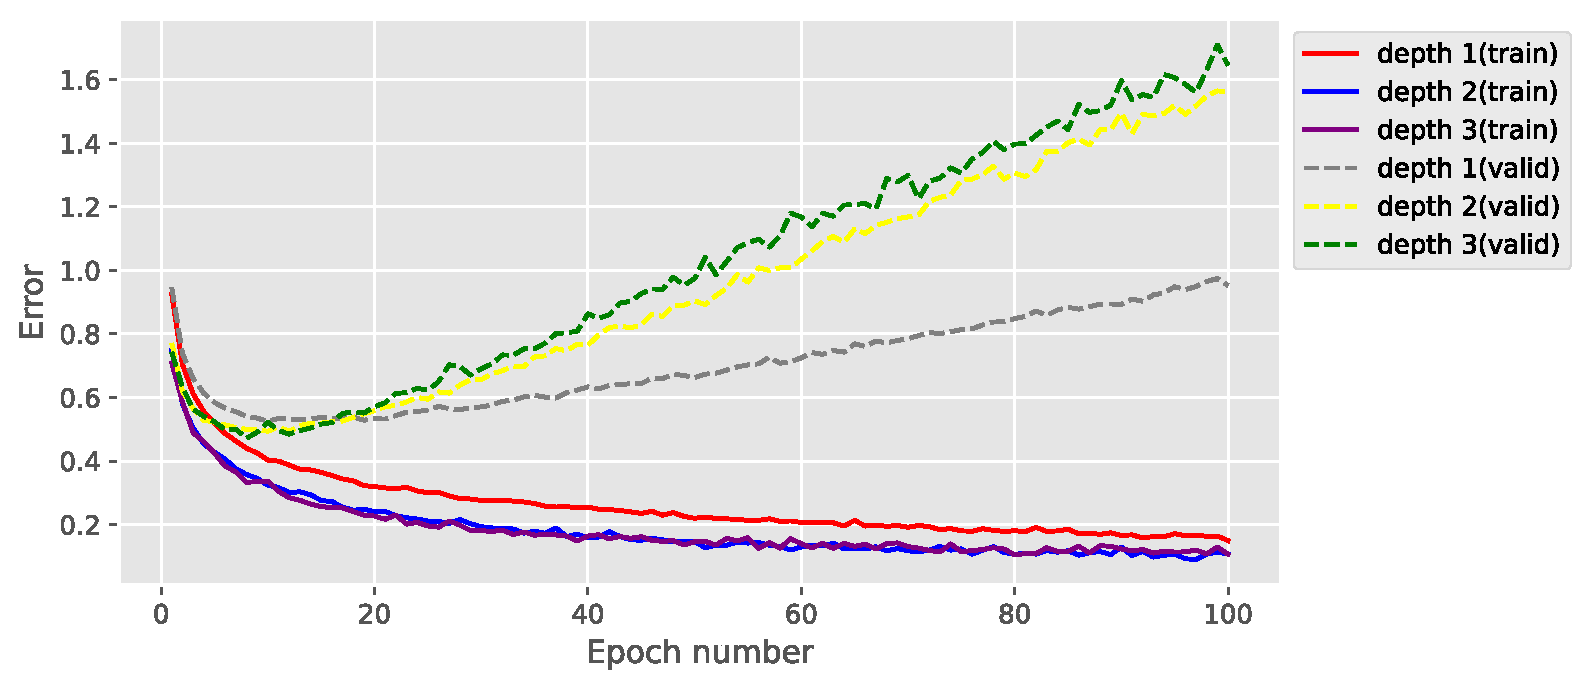
\includegraphics[width=\linewidth]{figures/depth-fig2.pdf}
        \caption{error by epoch}
        \label{fig:depth_errorcurves}
    \end{subfigure} 
    \caption{Training and validation curves in terms of classification accuracy (a) and cross-entropy error (b) on the EMNIST dataset for different network depths.}
    \label{fig:depth}
\end{figure} 
}
}

%% Question Figure 4:
\newcommand{\questionFigureFour} {
\youranswer{Question Figure 4 - Replace these images with figures depicting the Validation Accuracy and Generalisation Gap for each of your experiments varying the Dropout inclusion rate, L1/L2 weight penalty, and for the 8 combined experiments (you will have to find a way to best display this information in one subfigure).
%
\begin{figure*}[t]
    \centering
    \begin{subfigure}{.3\linewidth}
        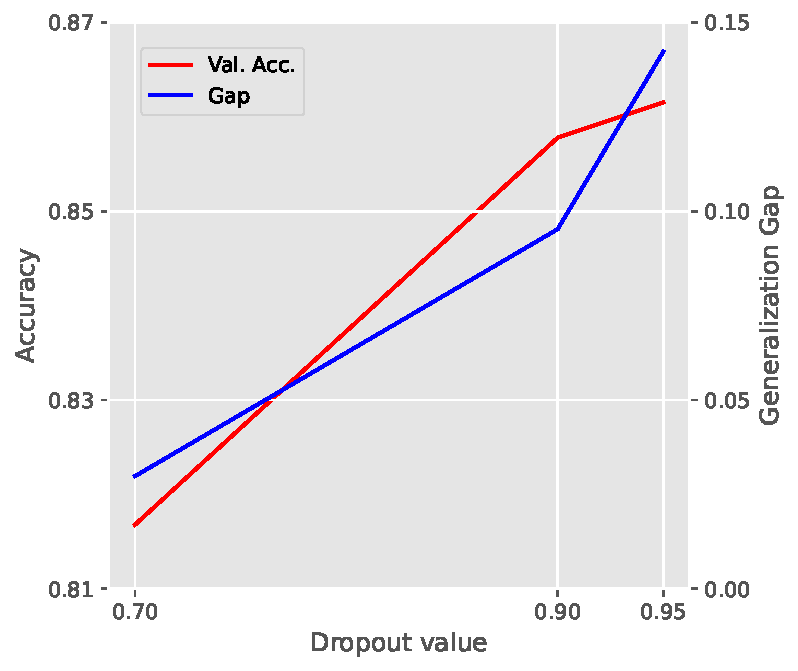
\includegraphics[width=\linewidth]{figures/dropout-val-acc-gen-gap-scaled.pdf}
        \caption{Metrics by inclusion rate}
        \label{fig:dropoutrates}
    \end{subfigure} 
    \begin{subfigure}{.3\linewidth}
        \centering
        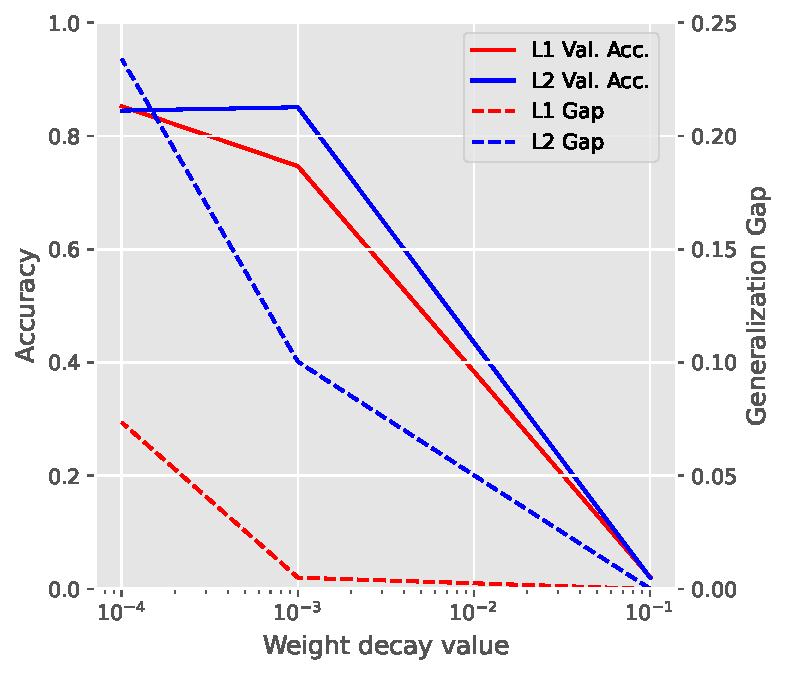
\includegraphics[width=\linewidth]{figures/l1-l2-val-acc-gen-gap.pdf}
        \caption{Metrics by weight penalty}
        \label{fig:weightrates}
    \end{subfigure} 
    \begin{subfigure}{.3\linewidth}
        \centering
        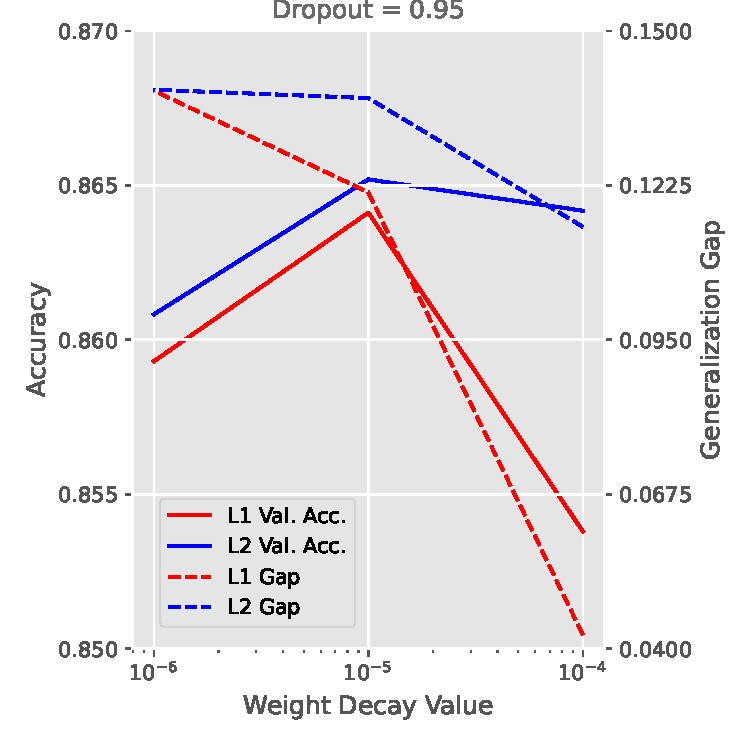
\includegraphics[width=1\linewidth]{figures/combined-val-acc-gen-gap-line.pdf}
        \caption{Metrics by combining inclusion rate and weight penalty}
        \label{fig:extra}
    \end{subfigure} 
    \caption{Hyperparameter search for every method and combinations}
    \label{fig:hp_search}
\end{figure*}
}
}

%% - - - - - - - - - - - - TABLES - - - - - - - - - - - - 

%% Question Table 1:
\newcommand{\questionTableOne} {
\youranswer{
%Question Table 1 - Fill in Table 1 with the results from your experiments varying the number of hidden units.
%
\begin{table}[t]
    \centering
    \begin{tabular}{c|cc}
    \toprule
        \# hidden units & val. acc. & generalization gap \\
    \midrule
         32            &      77.94\%      &      0.148              \\
         64            &      80.91\%      &      0.344              \\
         128           &      80.92\%      &      0.803              \\ 
    \bottomrule
    \end{tabular}
    \caption{Validation accuracy (\%) and generalization gap (in terms of cross-entropy error) for varying network widths on the EMNIST dataset.}
    \label{tab:width_exp}
\end{table}
}
}

%% Question Table 2:
\newcommand{\questionTableTwo} {
\youranswer{
%Question Table 2 - Fill in Table 2 with the results from your experiments varying the number of hidden layers.
%
\begin{table}[t]
    \centering
    \begin{tabular}{c|cc}
    \toprule
        \# hidden layers & val. acc. & generalization gap \\
    \midrule
         1               &      80.92\%      &    0.803               \\
         2               &      81.56\%      &    1.456               \\
         3               &      82.51\%      &    1.538               \\ 
    \bottomrule
    \end{tabular}
    \caption{Validation accuracy (\%) and generalization gap (in terms of cross-entropy error) for varying network depths on the EMNIST dataset.}
    \label{tab:depth_exps}
\end{table}
}
}

%% Question Table 3:
\newcommand{\questionTableThree} {
\youranswer{
Question Table 3 - Fill in Table 3 with the results from your experiments varying the hyperparameter values for each of L1 regularisation, L2 regularisation, and Dropout (use the values shown on the table) as well as the results for your experiments combining L1/L2 and Dropout (you will have to pick what combinations of hyperparameter values to test for the combined experiments; each of the combined experiments will need to use Dropout and either L1 or L2 regularisation; run an experiment for each of 8 different combinations). Use \textit{italics} to print the best result per criterion for each set of experiments, and \textbf{bold} for the overall best result per criterion.
%
\begin{table*}[t]
    \centering
    \begin{tabular}{c|c|cc}
    \toprule
        Model    &  Hyperparameter value(s) & Validation accuracy & Generalization gap \\
    \midrule
    \midrule
        Baseline &  -                    &               0.836 &                 0.290 \\
    \midrule
        \multirow{3}*{Dropout}
                 & 0.7                   &   81.68\%                   &  \emph{0.030}    \\
                 & 0.9                   &   85.78\%   &  0.095           \\
                 & 0.95                  &   \emph{86.15\%}                   &  0.142           \\
    \midrule
        \multirow{3}*{L1 penalty}
                 & 1e-4                   &  \emph{85.25}\%                   &  0.074           \\
                 & 1e-3                   &  74.67\%                   &  0.005           \\
                 & 1e-1                   &  2.11\%                    &  \textbf{\emph{0}}               \\
    \midrule
        \multirow{3}*{L2 penalty}  
                 & 1e-4                   &  84.47\%                   & 0.234            \\
                 & 1e-3                   &  \emph{85.07}\%                   & 0.100            \\
                 & 1e-1                   &  1.98\%                   & \textbf{\emph{0}}                \\
    \midrule
        \multirow{6}*{Combined}  
                 & 0.95, L1 1e-4  &      85.38\%               &   \emph{0.042}                  \\
                 & 0.95, L1 1e-5                    &     86.41\%                &              0.121           \\
                 & 0.95, L1 1e-6                   &    85.93\%                 &      0.139                   \\
                 & 0.95, L2 1e-4                   &     86.42\%                &      0.115                   \\
                 & 0.95, L2 1e-5                   &   \textbf{\emph{86.52\%}}                  &      0.138                   \\
                 & 0.95, L2 1e-6                   &  86.08\%                  &      0.140                   \\
    \bottomrule
    \end{tabular}
    \caption{Results of all hyperparameter search experiments. \emph{italics} indicate the best results per series and \textbf{bold} indicate the best overall}
    \label{tab:hp_search}
\end{table*}
}
}

%% END of YOUR ANSWERS